\documentclass[11pt,pdftex,twocolumn]{article}
\usepackage{alltt}
\usepackage[dvips]{graphicx}
\usepackage{verbatim}
\usepackage[margin=1in, paperwidth=8.5in, paperheight=11in]{geometry}
\usepackage{url}

\title{Watt's Happening}
\author{Ben Bramble, Nick Burek, Alexis Fisher, and Adam Vail}
\begin{document}
\maketitle

%TODO abstract
% abstract should include something about "created Watt's Happening"
\begin{abstract}
% motivation
% The 
% Ubiquitous mobile devices 
%    widening gap between device computing power and battery technology
Unfortunately, short battery life severely limits the full potential of mobile devices.
%Widespread use of mobile devices has 
%Mobile devices are prominent, but battery technology is lagging behind.
%Batteries constrain device use more than other hardware, as power draw increases.
% design 

These issues inspired our creation of \emph{Watt's Happening}, an Android application that aids users in maximizing their device's battery life.
% evaluation results
% conclusion

\end{abstract}
\section*{Introduction}
\label{sec:intro}
This paper describes the \emph{Watt's Happening} battery monitoring application. 
With the rapid increase in the prevalence of mobile device technology into everyday usage, users want to be sure that their device will not die in the middle of the day.
This can be tricky to balance since it's not always immediately apparent where the energy is getting spent in your device.
\emph{Watt's Happening} tracks the hardware state, battery level changes, and application resource usage. 
This data is used to compile resource usage metrics, providing information to the user on how much longer their device will last at their current rate.
By providing the user with this aggregated information in an easy to comprehend manner, users are able to make more informed decisions about how best to maximize their battery life.

\section*{Motivation}

\section{Design}
\label{sec:design}
%\subsection*{Assumptions}
%	short-running processes will have their battery usage amortized over longer running apps.
% could check all apps (instead of just running apps at snapshot),
% but balance between WH's power usage and ability to provide useful info to end user.
% 
% Assume that apps that use significant power will be spotted eventually, unless waking up on strictly opposite cycle.
% Assume short-term information more informative than historic view -- analyzer assumes current behavior will continue
% analyzer examines CPU and network I/O.  Due to time constraints, these metrics are currently separated.  Future work could provide a unified metric of usage.

%%
% why do we believe we will eventually see short-running apps?
% because if they're drawing significant battery and we don't see them,
% chances are high the app is 'hiding' itself from WH
% since apps that 
% 1) short term apps get bg'd not killed
% 2) most apps are user-driven, so not strictly cyclical (so not opp WH cycle)
% 3) in general, short-term apps won't use much power
%     so for power depletion to be significant, must run very frequently
% energy draw is amortized over all running apps

The \emph{Watt's Happening} application provides an estimate of remaining battery time, based on current and historic resource usage metrics. 
Our application provides an estimate along with a list of the currently running applications, weighted based on resource usage metrics.  
This provides the user with information that can be used to terminate a running application, thereby lengthening remaining battery time.
\emph{Watt's Happening} calculates the resource usage metrics on a per-application basis.
The resources examined include CPU and network I/O.
The reason to choose these resources for examination is twofold: the ease of measurement, and the high correlation between the use of these resources and battery draw.

We gather data from the underlying operating system in order to obtain metrics on resource usage.
The logging code queries and retains the status of hardware devices including radio states, location, screen state, and battery levels.
We query and retain currently running applications and resource consumption metrics to attribute hardware use to each application.
For battery drain, we attribute the change in level to hardware states.
Application use of hardware allows allocation of battery consumption across applications.
Of course, the act of measuring carries the risk of excessive power draw; we attempt to obtain representative data collection in a power conserving manner.
Performing this balance does allow the possibility that short-running applications will not be seen by the \emph{Watt's Happening} logger.
We assume that short-running applications that account for significant battery draw will eventually appear to our logger.
This is a reasonable assumption for several reasons.
First, most applications are not killed but simply backgrounded and therefore run at the same time as the logger.
Generally, user-driven applications are not backgrounded.
%Unless the user only interacts with the application in cycles directly opposing the logger...
Unless the user only interacts with the application in cycles directly opposing the logger (which is unlikely), then at some point the logger will observe the application.
A frequently running application will eventually overlap with the logger.
Applications that are not visible to our logger will draw battery, but usage will be amortized over visible applications by necessity.


\emph{Watt's Happening} provides a battery life estimate based on rate of usage in conjunction with battery level remaining.
Recent activity strongly biases this estimate in its favor, while still incorporating long-term historic usage in certain scenarios.
Since the battery consumption rate is derived from the assumption that the current usage pattern will continue, recent activities will yield a more conservative estimation of future use.
%We use this assumption to find 
The reported time remaining requires a conservative estimate because user expectation dictates that the battery will last at least as long as the \emph{Watt's Happening} estimate.

%In the case of no change in the battery level during a short term snapshot, a longterm averaged estimate is used.

If the user desires to prolong their battery further than the estimate, \emph{Watt's Happening} presents a set of lists showing running applications sorted by respective resource usage.
Usage is directly tied to battery draw as described above. 
This allows the user to select what action to take (i.e., termination of one or more applications) to extend battery life by drawing attention to applications that are (i) currently running and (ii) drawing proportionally significant power.


%Time-biased battery life estimate 


%%%%%
%Before starting on the application, we made two design assumptions.  
%First, any services that end quickly will not be incorporated into the analysis.  
%We assume that only long running programs will have a significant effect on the overall battery usage.  
%There exists the possibility for short, intense applications to game the system by terminating before our application's polling, but we ignore that possibility for now.  
%The second assumption is that we only display candidate applications for termination if they are currently running.  
%TODO 
%Future variation of the program can implement features that inform the user how much longer they can run their favorite applications while still reaching their target, but currently we limit our focus.


\section{Implementation}
\label{sec:implementation}
We implemented \emph{Watt's Happening} on Android OS version 4.0, API level $>$ 14. 
The Android OS provides a variety of APIs allowing access to application and hardware information.
Our application obtains information not exposed via the API directly from the underlying operating system.

\subsection{Logging}
\label{subsec:impl_logging}
When obtaining information, it is important to ensure \emph{Watt's Happening} remains relatively low-impact.
We accomplish this by using a time-based polling method of collecting data, as opposed to constant and intrusive observation.
The Managers provided in the Android API allow \emph{Watt's Happening} to obtain resource usage.
Battery level, GPS state, WiFi state, Bluetooth state, network connection and screen state are all collected and stored.
Application information including UID, name, network data transmitted and received, CPU usage, and runtime is collected and stored. 
%
While \emph{Watt's Happening} acquires application information from the Managers described above, the API does not expose CPU usage.
\emph{Watt's Happening} obtains CPU usage in the same manner as `top', `ps', and other standard system tools.
Each application contains a file in the proc directory that allows \emph{Watt's Happening} to collect the CPU ticks for the application.
%
Our application correlates this value to the number of overall CPU ticks to determine the percentage of the CPU the application consumed during the logging window.
\emph{Watt's Happening} polls every five minutes based on our iterative experiments.
We believe this maintains the delicate balance between fine-grained information capture and battery used by \emph{Watt's Happening}.
Time-based polling does not capture some low-duration, high-power events such as BlueTooth pairing and GPS-based events.
To handle these cases, our framework allows for event listeners.
Passive loggers capture these events when they occur.

\subsection{Analysis}
\label{subsec:impl_analysis}
\emph{Watt's Happening} collects data every five minutes, but delays analysis until sufficient information exists to justify the overhead of performing the analysis.
The analysis performs two distinct tasks, aggregating application resource usage and determining projected battery longevity.
Application CPU and network I/O information is condensed to a persistent long-term running average, and stored.
Once the analysis stores the average, the application archives the short-term information, thus reducing the memory footprint of our program.
\emph{Watt's Happening} projects the battery longevity estimate based on short and long term battery drain rate.
We calculate the drain by compiling the battery level change over time, yielding  percentage decrease in battery level per minute. 
Our application uses a non-zero short term drain rate whenever possible.
Since the device only reports the battery level to the closest 1\%, we may not observe a visible change over a short term period, especially with an idle device.
In this case, we estimate battery longevity based on the long term battery drain rate.
This allows for a highly responsive model based on changing usage patterns, while still maintaining accuracy over long term idle periods.
As demonstrated in Figure \ref{fig:bat_v_time}, naively using all collected data leads to averaging multiple disparate usage patterns, which can lead to gross overestimation.  
This motivates our choice to use solely short-term use information when available.
%Although we experimented with combining the short and long term rates, this failed to capture the impact of significant short term usage.  
%This would result in severe overestimation of remaining battery duration.
Future long term rates incorporate current short term usage if the device returns to an idle status.
\begin{figure}[ht!]
	\begin{center}
		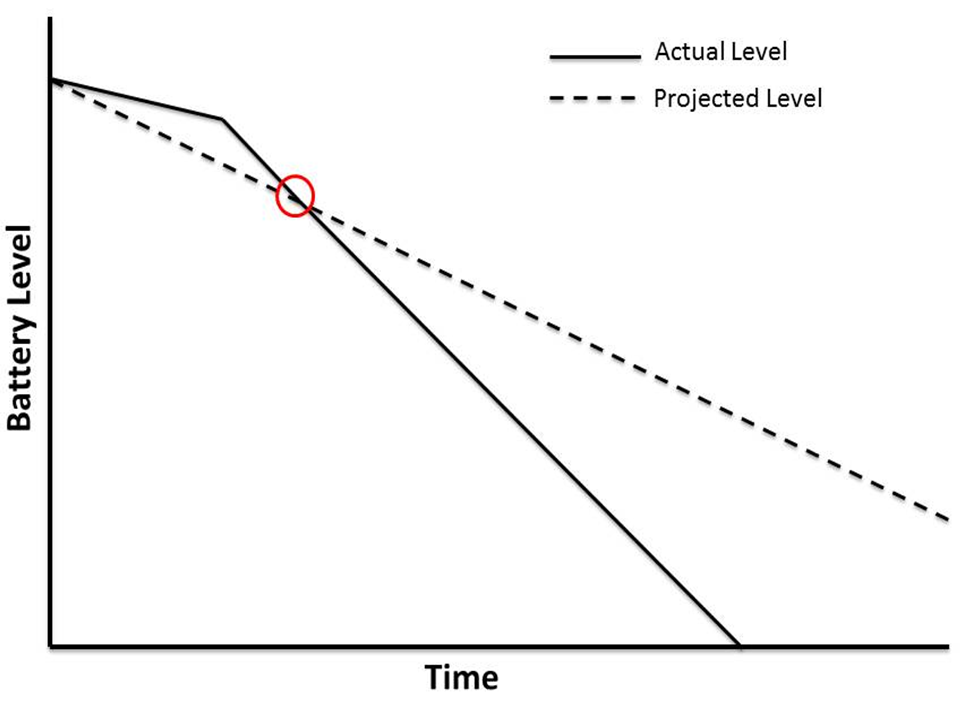
\includegraphics[width=\columnwidth]{figs/bat_vs_time.png}
		\caption{Actual battery depletion and projected depletion rate at analysis time}
		\label{fig:bat_v_time}
\end{center}
\end{figure}
% time remaining: battROC / time
% 

%%re-incorporate example?
% I like the example-- we should maybe provide it here or ? 
%   & not interspersed with implementation details
%   some sort of chart: time v. battery with prediction lines
% 
%Foremost, one must weigh the importance of recent data versus historic data.  
%A user's device usage rate is not likely to stay constant throughout the day.  
%For the majority of the day, the device might sit idle with occasional high power draining applications. 
%As a result, the long term usage rate alone cannot be the sole representation for analyzing and predicting the remaining time.  
%A common example would be a device that has been on idle for nearly a whole day.  
%The long term rate at this point would be a slow decrease that has left the phone low on remaining battery.  
%For the next five minutes, the user begins playing a CPU and network intensive game.  
%The user then wants to know if their device will last another hour.  
%If only the long term rate is used, that last five minute high usage rate is lost amongst the previous 24 hours.  
%However, the user is likely to continue running the game in the immediate future.  
%The long term collection and the most recent usage are combined with specific weights to create the most insightful recommendation possible. 
%With the overall rate and predicted end time determined, the application will be able to identify the primary culprits in the battery drain.  
%For our project, a culprit is an application that uses battery through intensive CPU or network use.  
%When the analyzer is started, Watt's Happening cycles through the list of currently running applications.  
%As stated in the assumptions section, only currently running applications are candidates for termination.  
%The analyzer considers the recent behavior as captured into the database and calculates the CPU and network use designated to each UID during the duration that it has been running.  
%With the CPU and network cost assigned to each culprit, the analyzer can determine the approximate cost of each culprit by combining those values with the amount of battery drained overall during the time period that the application was running.  
%The resulting value is used as a heuristic variable to allow comparisons between culprits and the follow-on recommendations to the user.
%\subsection*{Making Recommendations}
%The key to the success of Watt's Happening is arming the user with knowledge of their use and make knowledgeable recommendation to keep the device alive.  
%The logged information keep over a time period displaying the battery percentage versus time on a graph allows a graphical representation for the user to observe their usage habits. 
%The rate determined in the analyzer depicts on the graph the predicted battery termination time.  
%Should that time end before the user's goal, the application can display the top culprits currently running so the user is made aware of their candidates to close in order to reach their desired end time.
\subsection{Display} %TODO why we display what we do how we do dododo
Upon request, \emph{Watt's Happening} displays to the user currently running applications sorted by resource consumption.
This allows the user to see at a glance which applications are impacting their battery use rate. %change this
The user can then view the estimate of time remaining and decide to take action, including terminating a running application or continuing in their current state.

\section{Evaluation}
\label{sec:evaluation}
\begin{figure*}[ht!]
	\begin{center}
		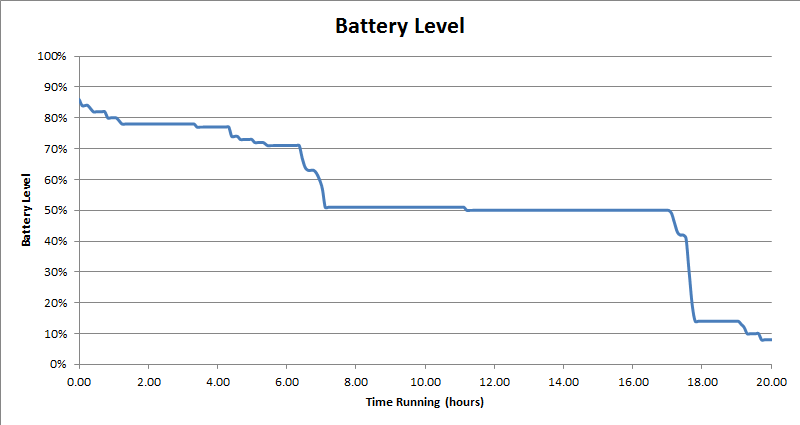
\includegraphics[scale=0.5]{figs/BatteryLevelLong.png}
		\caption{Battery Level Over Time, Dataset 1}
		\label{fig:bat_level}
\end{center}
\end{figure*}
\begin{figure*}[ht!]
	\begin{center}
		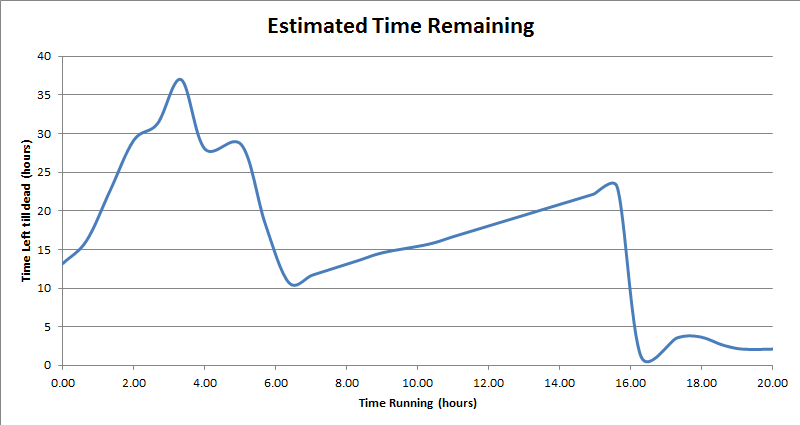
\includegraphics[scale=0.5]{figs/EstimatedTimeRemainingLong.png}
		\caption{Estimated Time Remaining Over Time, Dataset 1}
		\label{fig:est_remaining}
\end{center}
\end{figure*}
\begin{figure*}[ht!]
	\begin{center}
		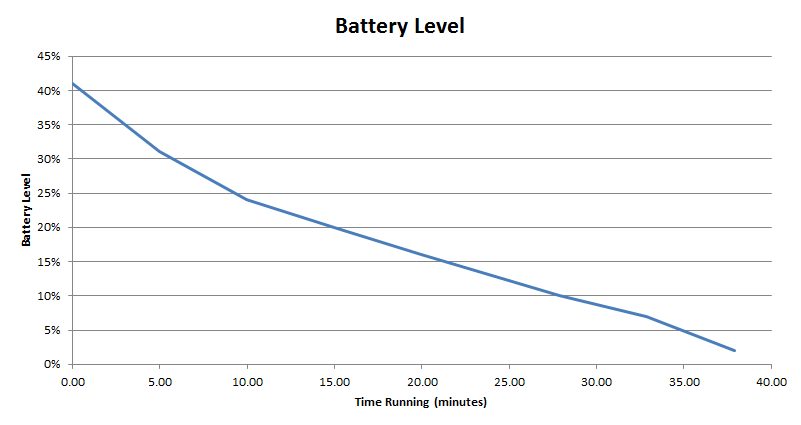
\includegraphics[scale=0.5]{figs/BatteryLevelShort.png}
		\caption{Battery Level Over Time, Dataset 2}
		\label{fig:bat_vs_time_short}
\end{center}
\end{figure*}
\subsection{Logging Window}
\emph{Watt's Happening} selected a five minute logging window.
This window was chosen to balance the impact on the system with a desire to capture as much data as possible, as mentioned in Section \ref{subsec:impl_logging}.
Our timing window also impacts our time remaining calculation, described in Section \ref{subsec:impl_analysis} 
As we've seen in our test cases, because battery level does not change for long periods of time while the phone idles, shorter logging windows would not provide more utility for our estimations. %TODO table ref
Using less than a five minute window, the number of short term observations with no battery change registered will grow, which results in more logging with no gain in useful data.
If more fine-grained battery information is required, we could register a \texttt{BatteryLevelChange} event handler to capture exactly when a battery level change occurs.
If we extend the logging window, there is a higher chance of missing applications that impact battery depletion.

\subsection{Estimation Model}
Initially, we experimented with using long term historical usage metrics in estimating application resource consumption.
This led to overestimation, since usage spikes are overly smoothed into long periods of near-zero resource consumption.
%This led to overestimation, since current usage is overly smoothed.
Next, we attempted to incorporate both long and short term usage metrics in estimating application resource consumption by doing a weighted average.
While our estimates improved, this still resulted in overestimation. 
Both overestimations were due to long periods with a lower rate of battery use outweighing short periods with a higher rate of battery use, which could continue until the end of the battery.
%This led to overestimation, since long periods with a lower rate of battery use outweighed the short periods with a higher rate of battery use that could continue until the end of the battery.
Due to our goal of not overestimating remaining battery levels, our estimation is derived primarily from short term use when available and falling back on historic usage information, as described in Section \ref{subsec:impl_analysis}.

\subsection{Experimentation}
% Methodology
Although formal and repeatable testing would have provided a consistent and controlled environment to display incontrovertible usage trends, a sterile environment is not the expected use case.
Therefore, averaging real world usage scenarios provides a more realistic, yet hopefully still convincing, data set.
We tested and analyzed \emph{Watt's Happening} via iterative real world testing on a selection of Android devices for over 40 hours of total testing time.
The devices included an HTC EVO 3D and a Motorola Droid RAZR both running Android 4.0. 

\subsection{Performance}
Figure \ref{fig:bat_level} shows the battery depletion over an approximately 20 hour run, beginning at approximately 11:00am. 
The long period of minimal battery depletion aligns with our test user's sleeping habits.
A sharp spike of device usage and corresponding battery depletion is evident, and correlates to our test user streaming music over 3G, a relatively resource intensive task.

Figure \ref{fig:est_remaining} is from the same test period as figure \ref{fig:bat_level}.
This figure shows \emph{Watt's Happening}'s estimate of remaining battery time, calculated every 30 minutes.
As we can see, over long idle periods our estimation tends to increase.
Conversely, over periods of heavy use, our estimation dramatically decreases in correlation with recent high usage.

Figure \ref{fig:bat_vs_time_short} shows the battery depletion over a 15 minute run.
The battery level drops from 50\% to 25\% over only 15 minutes, corresponding to our test user's use of a CPU-intensive game (in this case, \emph{Great Little War Game}\cite{glwg}).
At the end of this use session, Watt's Happening estimated  approximately 20 minutes of battery life remains if application use is continued.
This estimate is accurate, assessed by our test user continuing the activity until the device's battery was depleted.

Since the goal of \emph{Watt's Happening} is to monitor application resource usage, we can use  \emph{Watt's Happening} to monitor itself.
In our test runs, \emph{Watt's Happening} routinely uses a negligible amount of CPU resources, in relation to other running applications.
Therefore, we conclude that the resource consumption of \emph{Watt's Happening} is acceptable.
Although we, the developers of \emph{Watt's Happening}, have taken great strides toward conservative yet accurate battery life estimates, runs with long idle times may still have some amount of overestimation.
%
%When taken in context to the life of the universe, for example, over estimation by hours is a very small thing. 
%Humans don't live that long, anyway.
%Timey-Wimey   %that got away from you there
%
This is due to the averaging of historic data.  
Potential solutions include removing long periods of idle time from the averaged data or using exponential weighted moving averages to deemphasize periods of low use the further these periods are from the present.


\section{Related Work}
\label{sec:related}
Zwang et al.\cite{Zhang:2010:AOP:1878961.1878982} created a similar program in 2010 called PowerTutor that provides a power estimate to various hardware components and then assigns power usage to specific applications.  
They created the benchmarks using a previous project call PowerBooter that monitored power consumption while controlling power management for individual components. 
Since their models are based off of specific hardware components, their application is intrinsically tied to specific devices.
They warn that if PowerTutor is used with devices other than their target devices, ``power consumption estimates will be rough."
\emph{Watt's Happening} is intended to be a more general application that can provide useful information to a user regardless of their device's hardware. 
PowerTutor ultimately allows developers to determine the impact of their own application to improve their software designs.  
Future work could seek to incorporate aspects of PowerTutor into Watt's Happening to fine-tune application usage details and improve recommendations.

Chang, Agrawal, and Cameron survey the power management techniques employed by Android and how popular applications abuse or take advantage of those techniques\cite{energy-aware}. 
They explore the idea that software written for mobile devices should be optimized for efficient power consumption, but in many cases the application developer doesn't necessarily take power into consideration. 
They do several case studies of popular applications and analyze how they interact with the CPU, the screen, and other aspects of the mobile devices. 
They came to the conclusion that even though Android does a great job to aggressively save power, application developers need to create their software with power consumption in mind. 
The paper is a beneficial overview of the Android power management system as well as several tools that can be used to monitor the power usage of a device's underlying hardware. 

Pathak, Hu, and Zhang help application developers create power conserving software through their energy profiling tool called \emph{eprof}\cite{Pathak:2012:ESI:2168836.2168841}. 
The tool allows developers to monitor power consumption with multiple granularities and determine which pieces of code consume the most energy. 
This is useful for catching programming bugs, such as holding onto a wakelock too long, as well as directing attention to code that needs to be optimized. 
It also illuminates the fact that large amounts of energy are used in I/O operations. 
This implies that in order to save energy it is important to only use 3G, GPS, and WiFi when it is truly necessary.
These observations led us to the conclusion that it is important for \emph{Watt's Happening} to record and correlate network usage to specific applications.
Also, since network operations were shown to be energy intensive, a recommendation system should place an emphasis on applications that abuse the device's networking.
%Therefore, it is clear that disabling these aspects of a mobile device can make profound differences in battery life.

There has also been significant work that offers insights into user profiling and modeling.
Eventually, \emph{Watt's Happening} aspires to leverage user profiling to automatically control the power of different radios on the device. 
This would allow the application to prolong the battery life of a mobile device just by observing a user's usage patterns.
Intelligent models are necessary in order to keep the application from being too intrusive in user actions.
If the application's actions cause annoyance to the user, then they will refuse to use the application. 

Balajinath and Raghavan discuss learning user behavior to build a model of non-malicious user actions, with the intent to easily identify malicious users\cite{Balajinath:2001:IDT:2294491.2294970}. 
User activity is recorded, and a newness factor is used to help identify behavior out of the norm. 
A 500-command history was identified as the amount of history required to ensure maximum prediction accuracy. 

Fawcett et al. use usage profiling to detect cellular cloning fraud \cite{dataMiningFraudDetection}. 
While the idea of profiling users based on when and where they use services is similar to what we are trying to do, they are using this information for a much different application. 

Murmuria et al. develop a system for modeling power consumption on smartphone devices by collecting data on the wakelock drivers for a device's subsystem \cite{mobilePowerUsageMeasurements}. 
They break down the major subsystems (CPU, display, graphics, GPS, audio, and WiFi) and develop metrics by which power consumption can be determined for each subsystem. 
The paper provides a good overview of a low impact way of determining power consumption of individual components in a smartphone.
This correlation between subsystem and power consumption would allow for more powerful recommendations by \emph{Watt's Happening}.
\emph{Watt's Happening} could then give predictions stating how long a specific application can run while still achieving the overall battery-life goal for the device.

Goecks and Shavlik address unobtrusive observation of user behavior \cite{Goecks:2000:LUI:325737.325806}. 
Users don't need to necessarily identify successful results, but measurements of success can be inferred from properties of successful predictions. 
These properties should be observable without user interaction to assess likelihood of success. 

% I have no idea how to connect this to what we did
%Ashbrook learns significant locations and predicts user movement from GPS data \cite{Ashbrook:2002:LSL:862896.881068}. 
%Raw location data is analyzed using k-clustering with a variety of radiuses. 
%A building location is inferred from lack of GPS information for an arbitrarily selected ten minute time slice. 
%This is vulnerable to other GPS data issues, including urban canyons or device failure. 
%The location prediction is based on a Markov model built off of observed patterns. 
%First order Markov models are used, as data models beyond that would require a much longer observation period. 

Rumble et al. discussed a new operating system called Cinder that sought to extend limited energy resources by implementing capacitor objects \cite{Rumble:2009:AJT:1592606.1592618}. 
The similarities to their work included a desire to reach a goal usage time by dynamically running statistics of application energy consumption. 
The differences between their OS and our goal is that they built a new OS where as we aim to create an application on top of Android. 
In addition, Cinder actively limits the energy consumption of various applications where we will create suggestions for the user to implement. 

Zeng et al. established energy as a resource called currentcy and established pricing for using that resource \cite{Zeng:2003:CUA:1247340.1247344}. 
Both currentcy and Watt's Happening set usage time goals and dynamically adjusts to overspent and underspent energy to allow the application to meet that energy goal. 
However, currentcy forces all devices on the platform to adopt the energy resource type. 
This makes application programmers factor currentcy in to their design whereas Watt's Happening aims to be invisible to other applications. 

Shi et al. develop a method of identifying users based on behavior profiling \cite{learningUserBehavior}. 
Their methods of learning users' typical habits could be applied to power usage as well. 
If we know that a person uses their GPS when traveling to work every morning then we can account for that required power consumption when modeling usage goals. 

Oliner et al. develop Carat, a system to identify misbehaving code and energy-inefficient applications \cite{Oliner:2012:CED:2387858.2387864}.
Carat is differentiated from \emph{Watt's Happening} by using a community model.
Carat's sparse information gathering is also different than \emph{Watt's Happening}'s continuous logging cycle.
Due to this sparseness, Carat estimations of application usage may not be available to the user for up to a week after initial installation.
\emph{Watt's Happening} can provide preliminary observations after the first analysis has been performed, as quickly as 15 minutes after initial installation.

%%%%%%%%%%%%%%%%%%%%%%%%%
%
% thoughts on carat:
% carat uses sparse information, device (assuming therefore user) specific.
% can take up to a week to provide recommendations (as opposed to WH's hours)
% good ideas to cull: 
% 	confidence rating
% 	measure of similar devices (more difficult to define 'similar' w/android)
% 	
% 
%%%%%%%%%%%%%%%%%%%%%%%%%

\section{Future Work}
\label{sec:future}
\subsection{Power Model}
\emph{Watt's Happening} currently reports applications' use of hardware resources without linking resource usage directly to power draw.
A power model that correlates a specific resource's use to battery draw would allow battery depletion to directly link to the responsible application.
%This would enable 

\subsection{User Model}
Developing a model of usage for specific user/device pairings would allow finer-tuned use models.
A user with a strong routine of device use will currently see very conservative estimates from \emph{Watt's Happening}, especially if battery depletion is high immediately after a charge followed by a long period of relatively slow depletion. 
A well-designed user model could account for usage habits and incorporate this information into the recommendation engine.

\subsection{Recommendation Engine}
Currently, \emph{Watt's Happening} provides lists of applications weighted by specific resource consumption.
A more robust recommendation engine could provide a single list of recommended actions, incorporating the user model, the power model, and past recommendations taken.
Past recommendations accepted would indicate the user's flexibility and priorities for the device.
If the user does not want to terminate a particular program, recommending this action does not ultimately aide the user, even with a very resource and battery intensive application.



\section*{Conclusion}

\emph{Watt's Happening} demonstrates the potential for an application existing exclusively in user space to log and analyze the actions of other applications.  
The result is an application that aids users in extending the battery life of their mobile device.
It does this by tracking application usage of important resources such as CPU and network communications.
This provides the user with relevant short and long term resource usage compressed into an estimated time remaining.
If the user desires to extend that time remaining, \emph{Watt's Happening} conveniently displays the currently running applications sorted by resource usage.
Our application assists users' continuing demand for longer lasting mobile devices by indicating resource intense applications. \emph{Watt's Happening} assists the user in  


{\footnotesize \bibliographystyle{acm}
\bibliography{references}}



\end{document}
